%
% linear.tex
%
% (c) 2021 Prof Dr Andreas Müller, OST Ostschweizer Fachhochschule
%
\section{Lineare Rekursionsgleichung mit konstanten Koeffizienten
\label{buch:rekursion:section:linear}}
\rhead{Lineare Rekursionsgleichungen}
Die Funktionalgleichung der Gamma-Funktion, die im
Abschnitt~\ref{buch:rekursion:section:gamma} untersucht wurde,
hat die Form einer linearen Rekursionsgleichung
\[
\Gamma(x+1) = x\Gamma(x),\qquad \Gamma(1) = 1.
\]
Gleichungen, die Werte einer Funktion für verschiedene
Argument in Beziehung setzen, heissen {\em Funktionalgleichungen}.
\index{Funktionalgleichung}%
Es war überraschend schwierig, eine Lösung für Funktionalgleichung
der Gamma-Funktion für beliebige komplexe $x$ zu finden.
In diesem Abschnitt soll daher eine Klasse von Rekursionsgleichungen
näher untersucht werden, für die einfache Lösungen möglich sind.

\subsection{Lineare Differenzengleichungen}
Die Fibonacci-Zahlen sind definiert durch die lineare Rekursionsgleichung
\begin{equation}
F_{n+1\mathstrut} = F_{n\mathstrut} + F_{n-1\mathstrut},
\qquad
F_1=1,\quad F_0=0.
\label{buch:rekursion:eqn:fibonacci}
\end{equation}
Ganz ähnlich wie bei der Gamma-Funktion kann man auch hier die Frage
stellen, ob es eine Funktion $F(z)$ von komplexen Argument gibt derart,
dass
\begin{equation}
F(z+1) = F(z) + F(z-1), \qquad F(1)=1,\quad F(0)=0.
\label{buch:rekursion:eqn:fibonaccikomplex}
\end{equation}

\begin{aufgabe}
Gibt es eine Funktion
\[
F(z) = \sum_{k=0}^\infty a_k (z-z_0)^k
\]
derart, dass
\[
F(z+1) = F(z)+F(z-1)?
\]
\end{aufgabe}

Sind $F_1(z)$ und $F_2(z)$ Lösungen der Differenzengleichung, dann
sind beliebige Linearkombinationen $\lambda F_1(z) + \mu F_2(z)$
ebenfalls Lösungen.
Ausserdem ist $e^{2k\pi i}F(z)$ eine Lösung der Differenzengleichung,
es gibt also unendlich viele linear unabhängige Lösungen.

\subsection{Lösung mit Exponentialfunktionen}
Gesucht ist eine ganze Funktion, also eine Funktion
$F\colon\mathbb{C}\to\mathbb{C}$, die Lösung einer
Differenzengleichung
\begin{equation}
\sum_{k=0}^n a_kF(z+n)=0,
\end{equation}
mit $a_n\ne 1$.
ist.
Ein erfolgversprechender Ansatz ist $F(z)=e^{bz}=(e^b)^z$, da die
Exponentialfunktion eine ganze Funktion ist.
Die Differenzengleichung führt auf
\[
0
=
\sum_{k=0}^n
a_kF(z+n)
=
\sum_{k=0}^n
a_k e^{b(z+n)}
=
e^{bz}
\sum_{k=0}^n
a_k (e^b)^n.
\]
Gesucht ist also $a\in\mathbb{C}$ derart, dass $e^a$ eine Nullstelle
des charakteristischen Polynomes
\[
p(x) = \sum_{k=0}^n a_kx^k
\]
der Differenzengleichung ist.
Die Zahl $a$ ist nicht eindeutig, denn wenn $e^a$ eine Nullstelle ist,
dann ist $e^{a+2\pi i}=e^a$ eine Nullstelle.
Dies sind die einzigen Lösungen der Differenzengleichung.

Seien also $\lambda_j$ die Nullstellen von $p(x)$ mit $1\le j\le n$.
Dann gibt es komplexe Zahlen $b_j$ 
mit $-\pi < \operatorname{Im}b_j < \pi$ derart, dass $e^{b_j}=\lambda_j$.
Die Funktionen
\[
F_{jk}(z) = e^{2k\pi i z} e^{b_jz}
\]
sind Lösungen der Differenzengleichung.

\subsection{Komplexe Fibonacci-Zahlen}
Matt Parker vom Youtube-Kanal Stand-up Maths hat in einem
Video\footnote{\url{https://youtu.be/ghxQA3vvhsk}} die Lösungsfunktionen
für die Differenzengleichung der Fibonacci-Zahlen für beliebige
reelle und komplexe Argumente visualisiert.
Die Nullstellen des charakteristischen Polynoms
\[
\lambda^2-\lambda-1=0
\qquad
\Rightarrow
\qquad
\lambda_\pm = \begin{cases}
\displaystyle
\frac{1+\sqrt{5}}{2}=\varphi
\\[8pt]
\displaystyle
\frac{1-\sqrt{5}}{2}=-\frac{1}{\varphi},
\end{cases}
\]
dabei ist $\varphi$ das Verhältnis des goldenen Schnittes.
Die Anfangsbedingungen $F(0)=0$ und $F(1)=1$ bedeutet, dass
\begin{equation}
F(z) = \frac{1}{\sqrt{5}}\varphi^z - \frac{1}{\sqrt{5}}\frac{1}{(-\varphi)^z}
\label{buch:rekursion:linear:fibonaccifunktion}
\end{equation}
Dies ist die Funktion, die Matt Parker in seinem Video visualisiert hat.
\begin{figure}
\centering
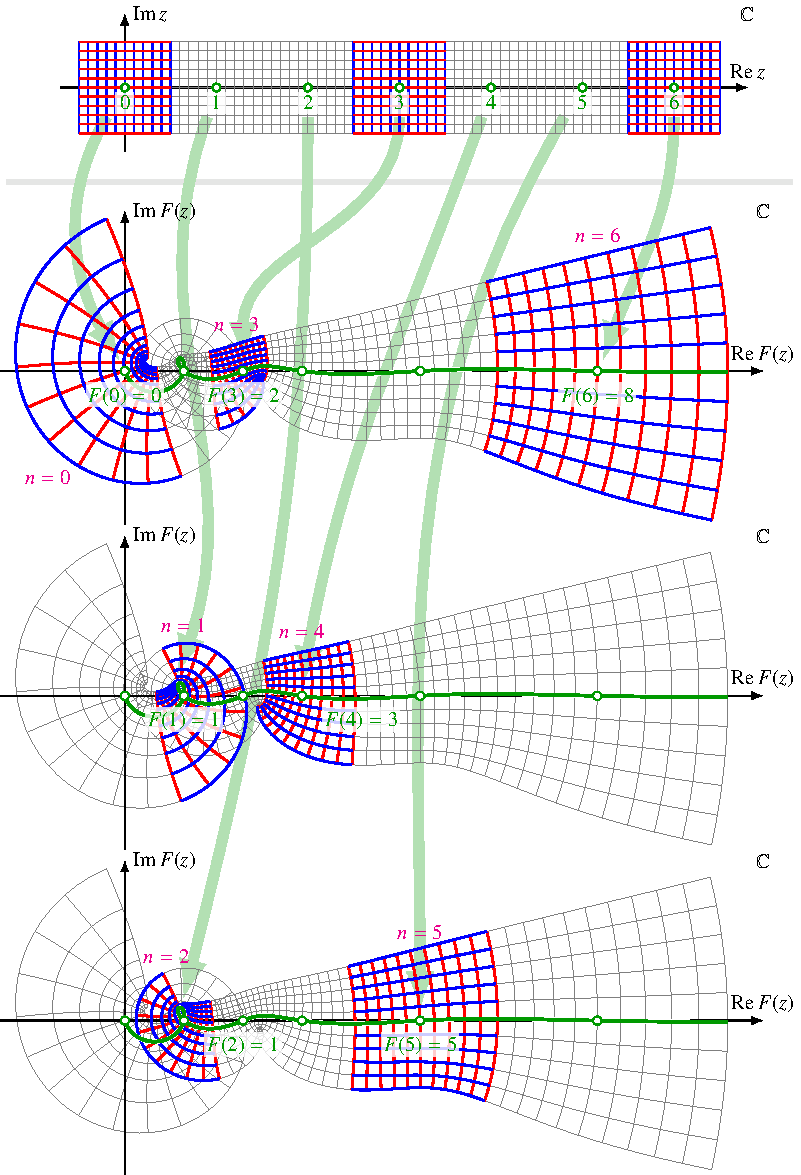
\includegraphics[width=0.82\textwidth]{chapters/040-rekursion/images/fibonacci.pdf}
\caption{Komplexe Fibonacci-Zahlen-Funktion $F(z)$ von
\eqref{buch:rekursion:linear:fibonaccifunktion}
dargestellt als Abbildung $\mathbb{C}\to\mathbb{C}$.
Die ganzzahligen $z$ werden auf die wohlbekannten Fibonacci-Zahlen
abgebildet.
Zur besseren Lesbarkeit wird der Wertebereich dreimal dargestellt,
damit die Bilder der einzelnen reellen Teilintervalle in verschiedene
Wertebereich-Bilder verteilt werden können.
$x$-Werte zwischen $3n-\frac12$ und $3n+\frac12$ werden im obersten
Bildbereich dargestellt, solche zwischen $3n+\frac12$ und $3n+\frac32$ 
im mittleren und schliesslich solche zwischen $3n+\frac32$ und $3n+\frac52$
im untersten.
Die reelle Achse wird auf die grüne Kurve abgebildet.
\label{buch:rekursion:linear:fibonaccigraph}}
\end{figure}
Abbildung~\eqref{buch:rekursion:linear:fibonaccigraph} zeigt die Abbildung
$z\mapsto F(z)$.
Allerdings sind die Funktionen
\[
F_{kl}(z)
=
\frac{1}{\sqrt{5}}
\varphi^ze^{2k\pi iz}
-
\frac{1}{\sqrt{5}(-\varphi)^z} e^{2l\pi z}
\]
ebenfalls Lösungen der Differenzengleichung mit den gleichen 
Anfangswerten.



